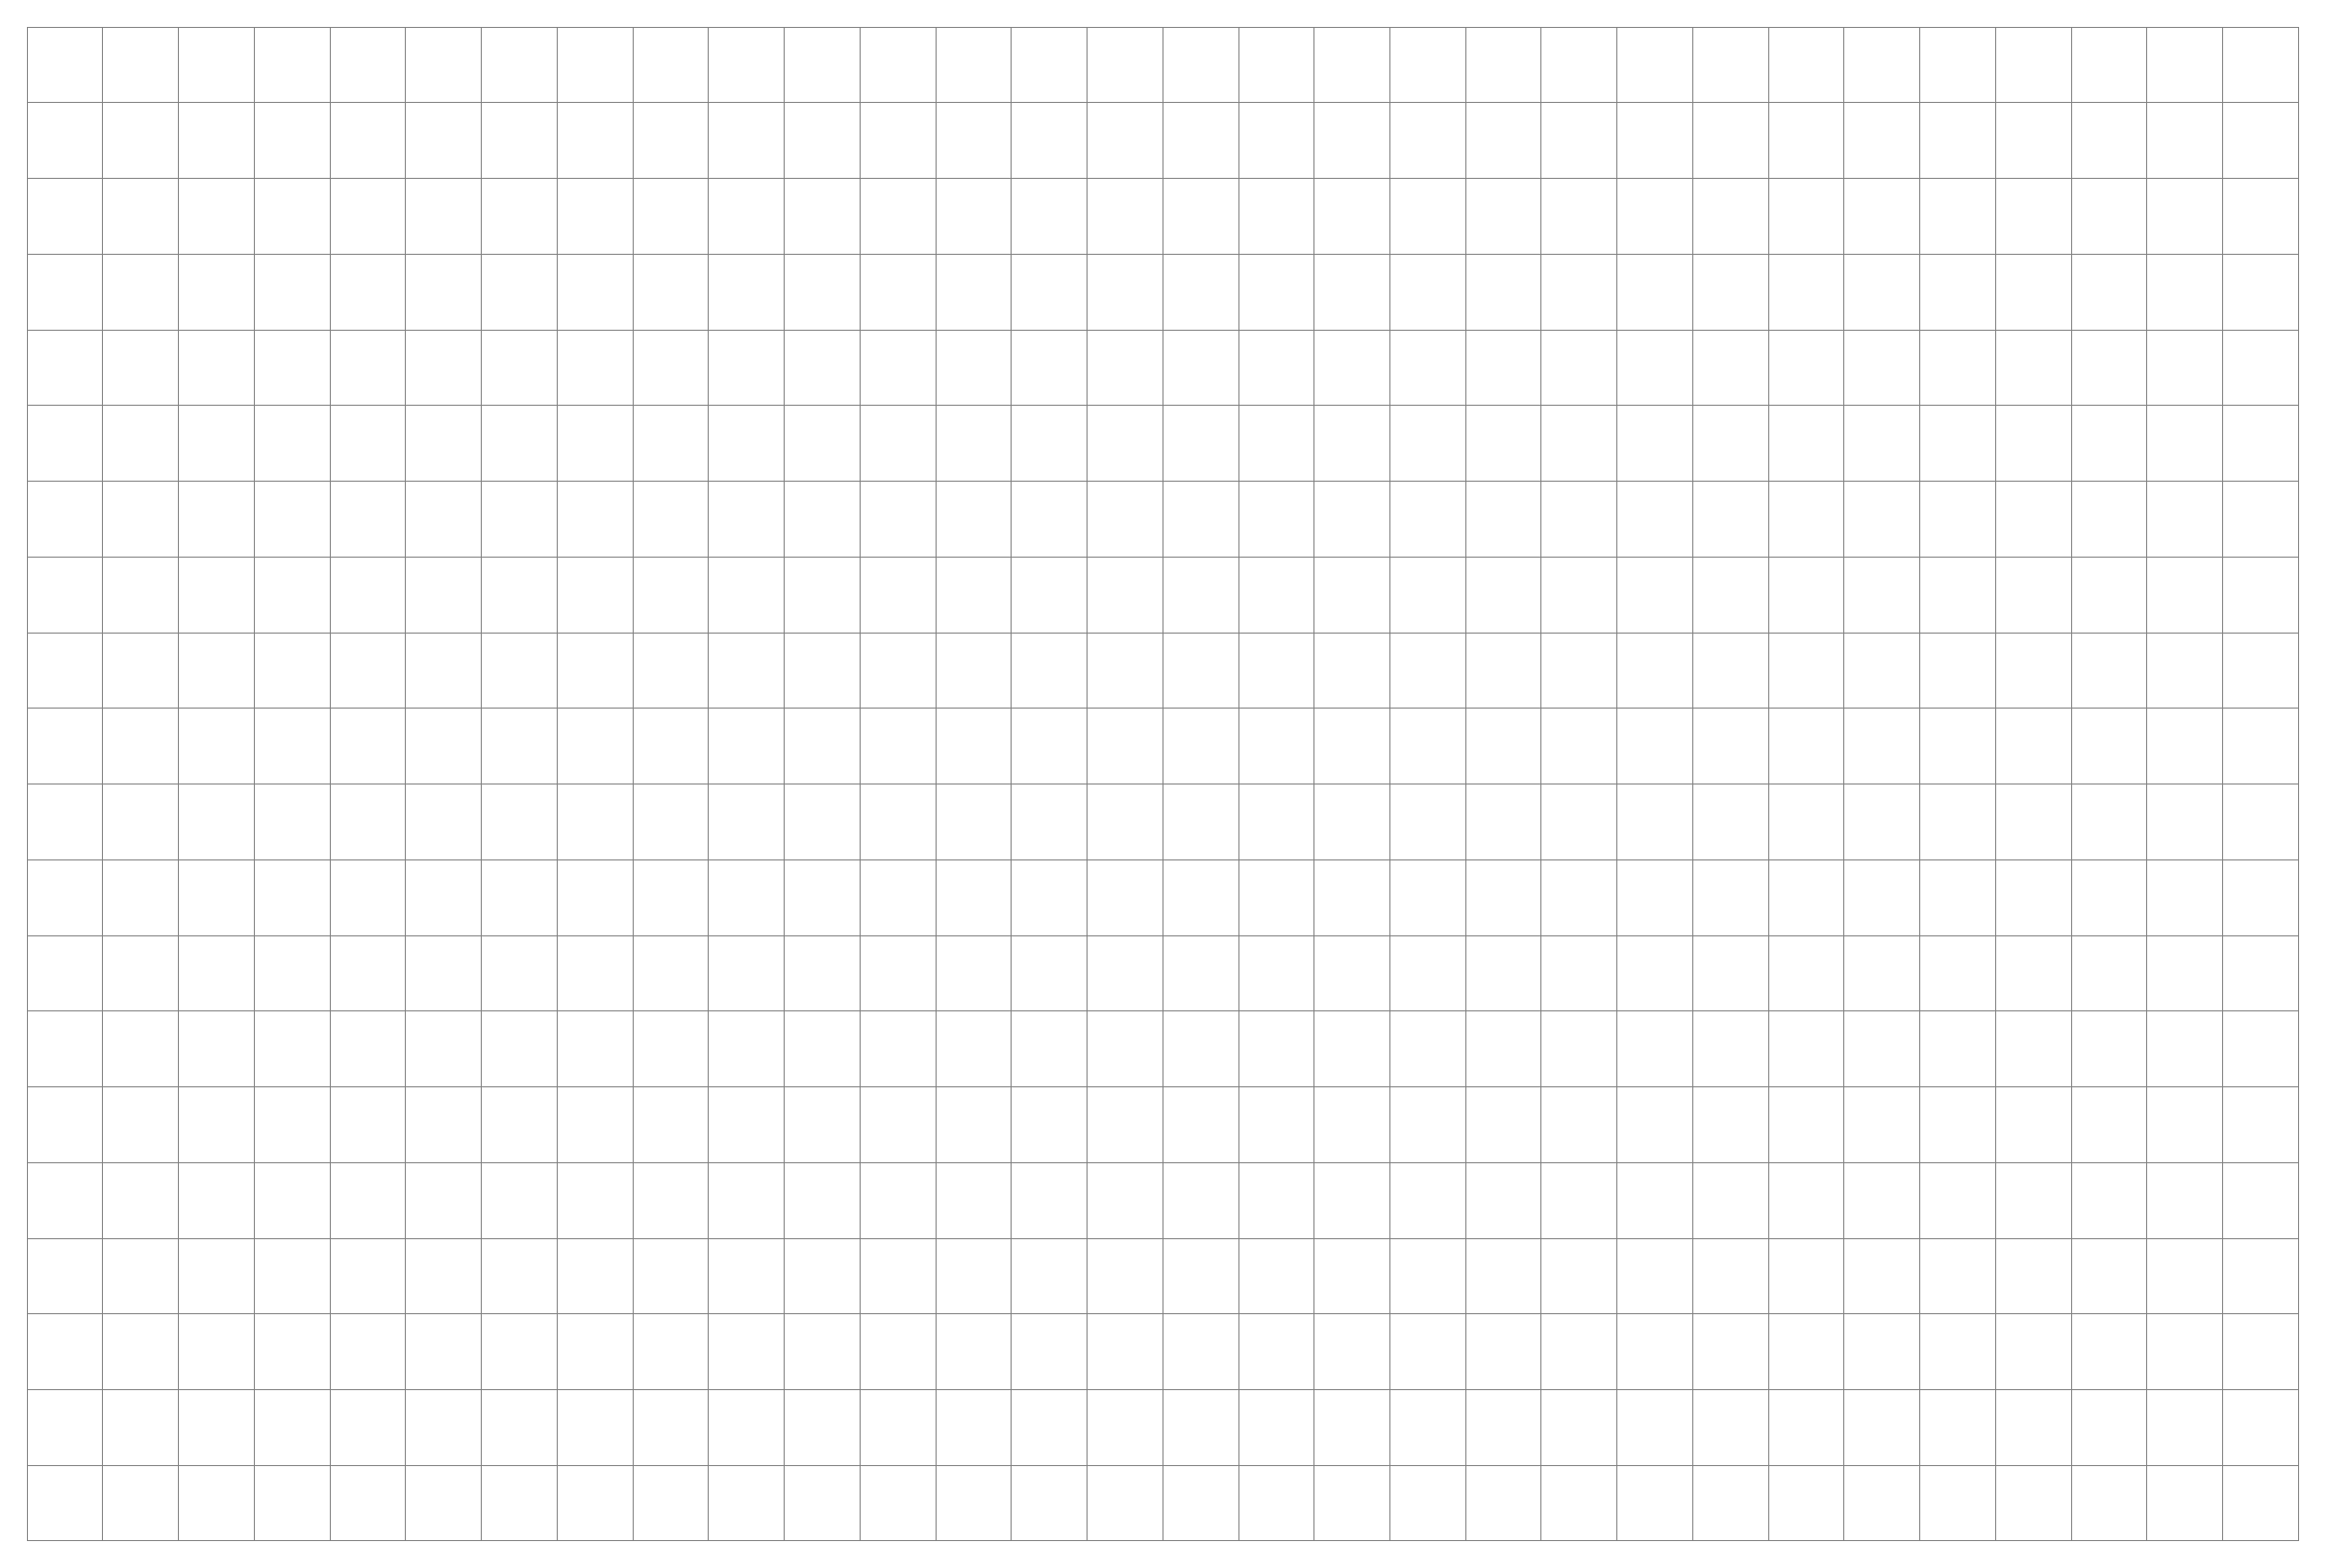
\begin{tikzpicture}

\GraphInit[vstyle=Classic]
\draw[help lines] (0,0) grid (30,20);

\begin{scope}[xshift=5cm, yshift=15cm]
\grComplete[prefix=q]{6}
\end{scope}

\begin{scope}[xshift=15cm, yshift=15cm]
\grComplete[prefix=q]{6}
\end{scope}

\begin{scope}[xshift=25cm, yshift=15cm]
\grComplete[prefix=q]{6}
\end{scope}

\begin{scope}[xshift=5cm, yshift=5cm]
\grComplete[prefix=q]{6}
\end{scope}

\begin{scope}[xshift=15cm, yshift=5cm]
\grComplete[prefix=q]{6}
\end{scope}

\begin{scope}[xshift=25cm, yshift=5cm]
\grComplete[prefix=q]{6}
\end{scope}

\end{tikzpicture}
